%! TEX root = ../main.tex
% ============================================================
% IMMUTABLE — generated automatically, do not edit this block
%   script          : plotter.py
%   plot_type       : ch04_mooring_comparison
%   chapter         : 04
%   panel           : None
%   wind            : None
%   amplitude       : None
%   frequency       : None
%   probes          : None
%   draft           : True
%
% DATASETS:
%   PROCESSED-20260326-ProbePos4_31_FPV_2-tett6roof-under9Mooring-height100-lowrange
%   PROCESSED-20260327-ProbePos4_31_FPV_2-tett6roof-under9Mooring30-height100-lowrange
%
% SUBFIGURES AVAILABLE:
%   FIGURES/ch04_mooring_comparison.pdf
% ============================================================
\begin{figure}[htbp]
  \centering
  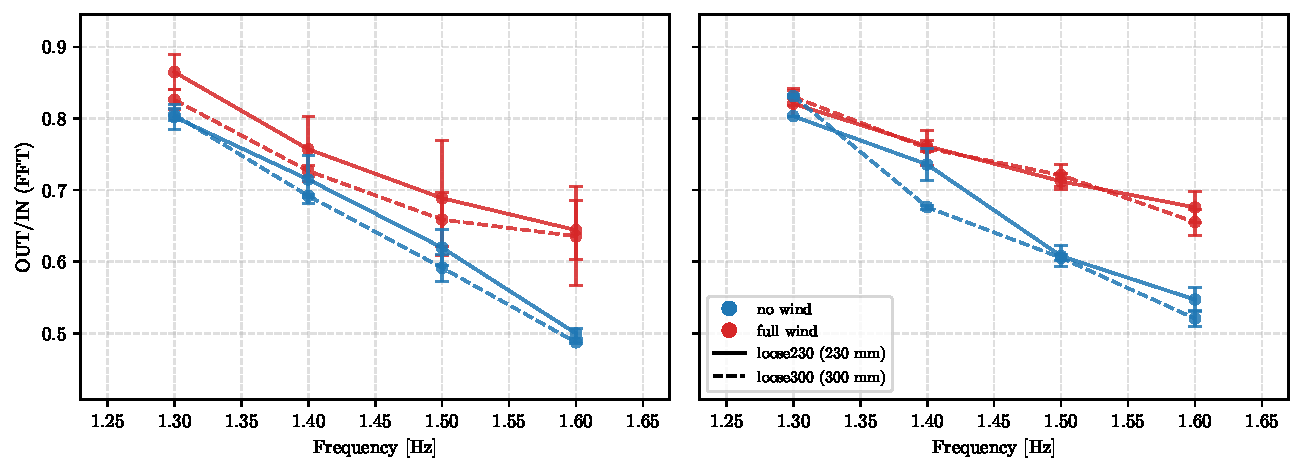
\includegraphics[width=0.9\linewidth]{FIGURES/ch04_mooring_comparison.pdf}
  \caption[OUT/IN(FFT) damping ratio at 0]{
    OUT/IN(FFT) damping ratio at 0.2\,V and 0.3\,V for two below-water mooring rubber band lengths: 230\,mm (blue) and 300\,mm (orange), both attached 90\,mm below the still-water surface. Solid lines: no-wind runs; dashed lines: full-wind runs. The two mooring types are indistinguishable within measurement uncertainty ($|\Delta| < 3\%$ at 1.4--1.6\,Hz, 0.2/0.3\,V). Panel geometry dominates wave transmission; mooring compliance does not. Datasets may therefore be merged as \texttt{below\_90\_loose} for result figures.
  }
  \label{fig:ch04_mooring_comparison}
\end{figure}
